\chapter{Configurazione dell'Ambiente}
\label{ch:env}
In questo capitolo descriviamo l'ambiente, le librerie e gli strumenti che utilizziamo per eseguire i nostri test.

Nelle sezioni seguenti installiamo gli SDK per sviluppare e interagire con i computer quantistici di IBM e D-Wave. Presentiamo inoltre altri due strumenti utili per scrivere facilmente problemi di ottimizzazione.

\section{Ambiente Python}
Il linguaggio usato per interfacciarsi con i computer quantistici è solitamente Python. In questa sezione creiamo un ambiente virtuale in Python per comunicare con il computer quantistico IBM e il computer quantistico D-Wave.

Per i nostri test gestiamo gli ambienti Python con \mintinline{sh}|conda|. Iniziamo creando l'ambiente virtuale denominato \mintinline{sh}|quantum| e attivandolo con:
\begin{center}
	\vspace{-.1cm}
	\begin{minipage}{.8\linewidth}
		\begin{minted}[linenos=false]{text}
			$ conda create --name quantum python=3.12 pip
			$ conda activate quantum
		\end{minted}
	\end{minipage}
\end{center}
Per i nostri test e per seguire i vari esempi presentati sia da IBM che da D-Wave, è utile anche poter eseguire un notebook Jupyter. Possiamo installare Jupyter con:
\begin{center}
	\vspace{-.1cm}
	\begin{minipage}{.6\linewidth}
		\begin{minted}[linenos=false]{text}
			$ pip install jupyter
		\end{minted}
	\end{minipage}
\end{center}

\section{IBM Qiskit}
Per programmare un'architettura basata su porte e per accedere ai computer quantistici IBM utilizziamo lo stack software \emph{Qiskit}. Il nome Qiskit è un termine generale che si riferisce a una raccolta di software per eseguire programmi su computer quantistici.
\begin{figure}[h]
	\centering
	
\includegraphics[width=.9\linewidth]{setup/overview-image}
	\caption{Stack software Qiskit}
	\label{fig:qiskit_overview}
\end{figure}

I componenti principali sono \emph{Qiskit SDK} e \emph{Qiskit Runtime}. Il primo è completamente open source e consente allo sviluppatore di definire il proprio circuito; il secondo è un servizio cloud per eseguire calcoli quantistici sui computer quantistici IBM.

\subsection{Hello World}
Seguendo la documentazione IBM\footnote{https://quantum.cloud.ibm.com/docs/en/guides/install-qiskit} possiamo installare l'SDK e il Runtime con:
\begin{center}
	\vspace{-.1cm}
	\begin{minipage}{.8\linewidth}
		\begin{minted}[linenos=false]{text}
			$ pip install qiskit matplotlib qiskit[visualization]
			$ pip install qiskit-ibm-runtime
			$ pip install qiskit-aer
		\end{minted}
	\end{minipage}
\end{center}

L'ultimo comando installa Aer, che è un simulatore ad alte prestazioni per circuiti quantistici scritti in Qiskit. Aer include modelli di rumore realistici, e lo utilizzeremo in seguito per testare il nostro circuito.

A volte lo stack Qiskit soffre di incompatibilità tra i vari componenti software che compongono l'ambiente. Al momento della stesura, gli ultimi pacchetti sembrano funzionare senza alcun problema. Per i nostri test utilizzeremo \mintinline{py}|qiskit: 2.2.3|, \mintinline{py}|qiskit-ibm-runtime: 0.43.1| e \mintinline{py}|qiskit-aer: 0.17.2|.

Se la configurazione ha successo siamo ora in grado di eseguire un piccolo test per costruire uno stato di Bell (due qubit entangled)\footnote{Otterremo lo stato $\Ket{\Psi^+}$ (Equazione~\ref{eqn:cnot})}. Il codice seguente assembla le porte, mostra il circuito finale e usa un sampler per simulare su CPU il risultato di $1024$ esecuzioni del programma.

\begin{listingenv}[h]
	\mylisting{.8}{py}{code/setup/hello_qiskit.py}
	\caption{Costruzione dello stato di Bell}
	\label{lst:hello_qiskit}
\end{listingenv}

\subsection{Transpilazione}
\label{sec:transpilation}
Ogni Unità di Elaborazione Quantistica (QPU) ha una topologia specifica. Dobbiamo riscrivere il nostro circuito quantistico per adattarlo alla topologia del dispositivo selezionato su cui vogliamo eseguire il nostro programma. Questa fase di riscrittura, seguita da un'ottimizzazione, è chiamata transpilazione.

Considerando un hardware finto (in modo da non necessitare di una chiave API) possiamo transpilare il circuito quantistico \mintinline{py}|qc|, dal codice precedente, per adattarlo alla topologia di una QPU specifica. Il Listato~\ref{lst:transpilation} implementa la transpilazione, e la Figura~\ref{fig:qc_transpilation} mostra i circuiti generati: (\hyperref[fig:qc_orig]{a}) è il circuito che abbiamo definito nel Listato~\ref{lst:hello_qiskit} e (\hyperref[fig:qc_trans]{b}) è la versione transpilata in cui la porta di Hadamard viene sostituita per adattarsi alla topologia effettiva della QPU.

\begin{listingenv}[h]
	\mylisting{.85}{py}{code/setup/transpilation.py}
	\caption{Transpilazione}
	\label{lst:transpilation}
\end{listingenv}

\begin{figure}[h]
	\centering
	\subfloat[Circuito originale]
	{\label{fig:qc_orig}
		
\includegraphics[height=2.8cm]{setup/bell_1}} \quad
	\subfloat[Circuito transpilato]
	{\label{fig:qc_trans}%
		
\includegraphics[height=2.8cm]{setup/bell_2}} \\
	\caption{Esempio di transpilazione}
	\label{fig:qc_transpilation}
\end{figure}

\subsection{Esecuzione}
Per testare il nostro circuito transpilato utilizziamo Aer, che ci permette di simulare anche il rumore dell'hardware quantistico reale. Il Listato~\ref{lst:execution} mostra come simulare l'esecuzione.
\begin{listingenv}[h]
	\mylisting{.9}{py}{code/setup/gate_execution.py}
	\caption{Esecuzione simulata}
	\label{lst:execution}
\end{listingenv}

Se\marginpar{Risultati con\\rumore simulato} osserviamo i risultati dell'esecuzione possiamo notare che alcune risposte presentano qubit non entangled; questo è causato dal rumore (simulato) del dispositivo quantistico. Un tipico output dell'esecuzione potrebbe essere:
\begin{center}
	\vspace{-.1cm}
	\begin{minipage}{.9\linewidth}
		\begin{minted}[linenos=false]{text}
			> counts Bell circuit: {'00': 504, '11': 503, '01': 10, '10': 7}
		\end{minted}
	\end{minipage}
\end{center}

Dove gli stati \mintinline{text}|01| e \mintinline{text}|10| non dovrebbero essere presenti in un'esecuzione ideale senza errori.

\section{D-Wave Ocean}
\label{sec:ocean}
Per definire un problema di ottimizzazione che può essere risolto su un computer quantistico D-Wave utilizziamo lo stack software Ocean. Ocean ci permette anche di interagire con l'hardware D-Wave, inviare un problema e simulare l'esecuzione su una CPU classica.
\begin{figure}[h]
	\centering
	
\includegraphics[width=.95\linewidth]{setup/ocean_stack}
	\label{fig:ocean_overview}
	\caption{Stack software Ocean}
\end{figure}

Tutti gli strumenti che implementano i passi necessari per risolvere il proprio problema su una CPU, un computer quantistico D-Wave o un solver ibrido quantistico-classico possono essere installati con:
\begin{center}
	\vspace{-.1cm}
	\begin{minipage}{.6\linewidth}
		\begin{minted}[linenos=false]{text}
			$ pip install dwave-ocean-sdk
		\end{minted}
	\end{minipage}
\end{center}

Dopo l'installazione, eseguendo il comando \mintinline{sh}|dwave setup| verrà avviato un prompt interattivo che ci guida attraverso una configurazione completa. Durante la configurazione è anche possibile aggiungere un token API o connettersi all'account D-Wave per importare direttamente una chiave per utilizzare l'hardware quantistico.

\subsection{Hello World}
Per presentare un semplice programma di ottimizzazione consideriamo il problema della copertura minima dei vertici (MVC). Dato un grafo $G = (V, E)$, il problema chiede di trovare un sottoinsieme $V' \subseteq V$ tale che, per ogni arco $\set{u,v} \in E$, almeno uno tra $u$ e $v$ appartenga a $V'$, e il numero di nodi in $V'$ ($|V'|$) sia il più basso possibile.

La\marginpar{MVC come problema\\di Ising} riduzione da MVC a una formulazione Ising è ben nota. La funzione di costo che vogliamo minimizzare può essere espressa da:
\[
cost = \sum_{i = 1}^{|V|}v_i + 2 \cdot \sum_{\set{i,j} \in E}\left(1 - v_i - v_j + v_i v_j \right)
\]
dove $v_i \in \set{-1, 1}$ e $v_i = 1$ significa che $v_i \in V'$, altrimenti $v_i = -1$.

Come tutti i problemi in forma Ising possiamo esprimere il costo come una matrice simmetrica, quindi la nostra funzione diventa
\[
cost = v^T \times \mathbf{M} \times v
\]
dove $v$ è il vettore contenente le variabili binarie $v_i$.

La figura mostra un grafo di esempio (\ref{fig:ising_ex_gr}) e la corrispondente matrice (\ref{fig:ising_ex_mx}) che esprime la funzione di costo.

\begin{figure}[h]
	\centering
	\subfloat[Grafo originale]
	{\label{fig:ising_ex_gr}
		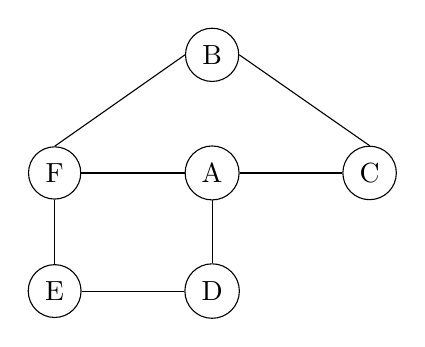
\begin{tikzpicture}
			\node (a) at (0,0)        [draw, circle] {A};
			\node (b) at (0,1.5)      [draw, circle] {B};
			\node (c) at (2,0)        [draw, circle] {C};
			\node (d) at (0,-1.5)     [draw, circle] {D};
			\node (e) at (-2,-1.5)    [draw, circle] {E};
			\node (f) at (-2,0)       [draw, circle] {F};
			\draw[-] (a.east)  -- (c.west);
			\draw[-] (a.south) -- (d.north);
			\draw[-] (a.west) -- (f.east);
			\draw[-] (b.east) -- (c.north);
			\draw[-] (b.west) -- (f.north);
			\draw[-] (d.west) -- (e.east);
			\draw[-] (e.north) -- (f.south);
		\end{tikzpicture}
	} \qquad
	\subfloat[Matrice corrispondente]
	{
		\label{fig:ising_ex_mx}%
		\begin{tikzpicture}
			\node (a) at (0,0) {
				$
				\mathbf{M} = 
				\begin{pmatrix}
					1&0&2&2&0&2\\
					0&1&2&0&0&2\\
					0&0&1&0&0&0\\
					0&0&0&1&2&0\\
					0&0&0&0&1&0\\
					0&0&0&0&0&1\\
				\end{pmatrix}
				$
			};
		\end{tikzpicture}
	}
	\caption{Formulazione Ising}
	\label{fig:ising_ex}
\end{figure}

Il\marginpar{Simulazione\\dell'esecuzione} codice seguente presenta una possibile implementazione del modello Ising descritto sopra. Abbiamo definito due dizionari per memorizzare i coefficienti della matrice. L'ultima riga di codice trova dieci possibili risposte al problema usando la funzione di simulated annealing implementata da D-Wave.
\begin{listingenv}[H]
	\mylisting{.9}{py}{code/setup/ising_ex.py}
	\caption{Esempio Ising}
	\label{lst:ising_ex}
\end{listingenv}

Se stampiamo i risultati con \mintinline{py}|print(result.aggregate())| possiamo osservare qualcosa di simile a questo:
\begin{center}
	\vspace{-.1cm}
	\begin{minipage}{.6\linewidth}
		\begin{minted}[linenos=false]{text}
			A  B  C  D  E  F energy num_oc.
			0 -1 -1 +1 +1 -1 +1  -14.0       6
			1 +1 +1 -1 -1 +1 -1  -14.0       4
			['SPIN', 2 rows, 10 samples, 6 variables]
		\end{minted}
	\end{minipage}
\end{center}
I due risultati diversi rappresentano le due risposte corrette alla nostra particolare istanza del problema MVC.

\section{PyQUBO e qubovert}
Nel Listato~\ref{lst:ising_ex} abbiamo costruito manualmente la matrice che rappresenta la funzione che vogliamo minimizzare. Può essere utile disporre di strumenti che ci permettano di lavorare a un livello più alto, definendo funzioni di costo come le Equazioni~\ref{eqn:ising} e \ref{eqn:qubo} che abbiamo definito nella sezione sul quantum annealing (Sezione~\ref{sec:annealing_form}).

Considerando di nuovo il problema MVC, la funzione obiettivo tende a minimizzare il numero di nodi nel nostro sottoinsieme, mentre la penalità aumenta il costo se tralasciamo alcuni archi. Questa interpretazione ci permette di trasformare il modello Ising nel modello QUBO più familiare \textemdash{}dal punto di vista di un informatico\textemdash{}, dove tutte le variabili $x_i \in \set{0, 1}$. Vediamo come PyQUBO e qubovert ci aiutano in questo compito.

\subsection{PyQUBO}
Leggendo dalla documentazione sul sito di PyQUBO\footnote{\url{https://pyqubo.readthedocs.io/en/latest/}}, PyQUBO ci permette di creare QUBO o modelli Ising da espressioni matematiche flessibili in modo semplice. Alcune delle caratteristiche di PyQUBO sono:
\begin{itemize}
	\item basato su Python (backend in C++);
	\item completamente integrato con Ocean SDK;
	\item validazione automatica dei vincoli;
	\item segnaposto per la regolazione dei parametri.
\end{itemize}

Possiamo installare PyQUBO con \mintinline{text}|$ pip install pyqubo| e riscrivere il nostro problema MVC definendo l'Hamiltoniano che vogliamo minimizzare.
\begin{listingenv}[h]
	\mylisting{.85}{py}{code/setup/mvc_pyqubo.py}
	\caption{Riscrittura del MVC con pyQUBO}
	\label{lst:MVC_pyQUBO}
\end{listingenv}

Il Listato~\ref{lst:MVC_pyQUBO} presenta una possibile reimplementazione del Listato~\ref{lst:ising_ex}, in cui vediamo anche come PyQUBO si interfaccia con Ocean SDK (riga 17), e come creare (righe 14–16) e istanziare (riga 17) un Hamiltoniano parametrico.

\subsection{qubovert}
Come scritto nella documentazione\footnote{\url{https://qubovert.readthedocs.io/en/latest/index.html}}, qubovert è il pacchetto unico per formulare, simulare e risolvere problemi in forma booleana e di spin. Usando la nostra nomenclatura, forma booleana e forma di spin sono rispettivamente la forma QUBO e la forma Ising.

Qubovert ci permette di definire vari tipi di problemi di ottimizzazione che possono essere risolti per forza bruta, con il simulated annealing di qubovert, o con il solver di D-Wave. I modelli definiti in qubovert sono:
\begin{description}
	\item [QUBO:] Ottimizzazione Booleana Quadratica Non Vincolata;
	\item [QUSO:] Ottimizzazione di Spin Quadratica Non Vincolata (modello Ising);
	\item [PUBO:] Ottimizzazione Booleana Polinomiale Non Vincolata;
	\item [PUSO:] Ottimizzazione di Spin Polinomiale Non Vincolata;
	\item [PCBO:] Ottimizzazione Booleana Polinomiale Vincolata;
	\item [PCSO:] Ottimizzazione di Spin Polinomiale Vincolata.
\end{description}

Oltre ai modelli generici, qubovert dispone di una libreria di famosi problemi NP-completi mappati nelle forme QUBO e Ising.

\begin{listingenv}[h]
	\mylisting{.85}{py}{code/setup/mvc_qubovert.py}
	\caption{Riscrittura del MVC con qubovert}
	\label{lst:MVC_qubovert}
\end{listingenv}

Il Listato~\ref{lst:MVC_qubovert} mostra una possibile implementazione del problema MVC usando gli strumenti forniti da qubovert. Qubovert ci permette di esprimere il nostro problema come PCBO; utilizziamo questa formulazione per esprimere i vincoli in modo più naturale. Nel nostro esempio ci assicuriamo che ogni arco sia coperto semplicemente imponendo che almeno uno dei nodi collegati dall'arco sia presente nella soluzione. Questo vincolo viene ripetuto per ogni arco del grafo (righe 7–13). I vincoli sono codificati nella funzione di costo usando una funzione di penalità moltiplicata per uno scalare: il \emph{moltiplicatore di Lagrange}. Per specificare il moltiplicatore di Lagrange usiamo la parola chiave \mintinline{text}|lam|.

Qubovert, come PyQUBO, può interfacciarsi con Ocean SDK, trasformando un problema PCBO in un problema QUBO (riga 15) e poi riscrivendolo nel formato accettato dal solver (o sampler) di D-Wave.

\section{Conclusione}
In questo capitolo abbiamo configurato un ambiente per eseguire i nostri futuri esperimenti e test. Abbiamo anche mostrato alcuni piccoli esempi per presentare le caratteristiche principali e testare gli strumenti che utilizzeremo nel nostro lavoro.

Seguire questa configurazione consente a chiunque di ricreare esattamente la stessa configurazione che utilizziamo, evitando (per quanto ne sappiamo e testiamo) incompatibilità tra i pacchetti Python.
